\chapter{RAID}
\label{ch:raid}

\section{RAID}
\label{sec:raid}

Redundant Array of Inexpensive Disks (RAID) is where a number of
identical standard drives are used in multiple. Depending on the
configuration used, this can increase capacity, performance and
reliability.

\begin{description}
\item[RAID levels]
are standard patterns in which RAID is implemented, .
\item[RAID set]
is a number of physical disks that has been combined using a RAID level.
A RAID set can be:

\begin{description}
\item[Healthy:]
where all of its member disks are working.
\item[Degraded:]
where one or more of its member disks have failed while the others
continue to work. I/O operations can continue.
\item[Failed:]
where one or more of its member disks have failed such that I/O
operations cannot continue.
\end{description}
\end{description}

\section{Metrics}\label{metrics}

\subsection{Fault tolerence}\label{fault-tolerence}

Each RAID level can tolerate a number of disks failing.

\subsection{Storage efficiency}\label{storage-efficiency}

The storage efficiency of a RAID set is:

\begin{verbatim}
E = ( useable capacity ) / ( sum of RAID set disks capacity )
\end{verbatim}

For any given RAID set, it depends on the RAID level, \texttt{L}, in use
and the number of disks, \texttt{n}.

\subsection{Write penalty}\label{write-penalty}

Most RAID levels have a write penalty, which is the number of write
operations that occur compared to when a single disk is used. A single
disk would have a write penalty of 1.

\section{Basic RAID levels}\label{basic-raid-levels}

The two basic RAID levels involve striping and mirroring. Assume that
some data has been split up into equally sized chunks labelled
\texttt{A1,\ A2\$} etc. Let \texttt{n} be the number of disks in the
set.

\subsection{RAID-0 (Stripe)}\label{raid-0-stripe}

RAID-0 splits, or stripes, data across a minimum of \(2\) disks, .

\begin{figure}
\centering
%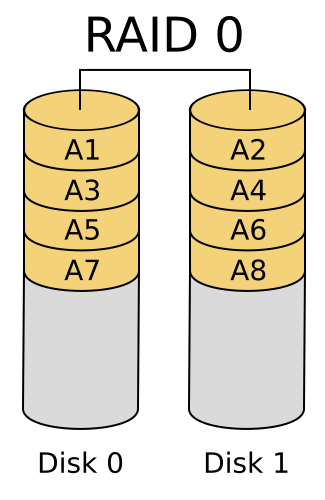
\includegraphics{RAID_0.svg}
\caption{RAID-0 with 2 disks}
\end{figure}

\subsubsection{RAID-0 fault tolerence}\label{raid-0-fault-tolerence}

RAID-0 has no fault tolerence. If any one disk fails no I/O can be
performed. If the failure is permanent, data is permanently lost.

Using standard redundancy notation, RAID-0 has redundancy \texttt{N}.

\subsubsection{RAID-0 storage
efficiency}\label{raid-0-storage-efficiency}

In RAID-0, data is striped across all disks in the set. The space of all
the \texttt{n} disks in the set is usable.

\begin{verbatim}
RAID-0 efficiency = n / n = 1
\end{verbatim}

\subsubsection{RAID-0 write penalty}\label{raid-0-write-penalty}

RAID-0 does not incur additional writes, so its write penalty is 1.

\subsection{RAID-1 (Mirror)}\label{raid-1-mirror}

RAID-1 mirrors, or copies, data across \texttt{n} disks:

\begin{figure}
\centering
%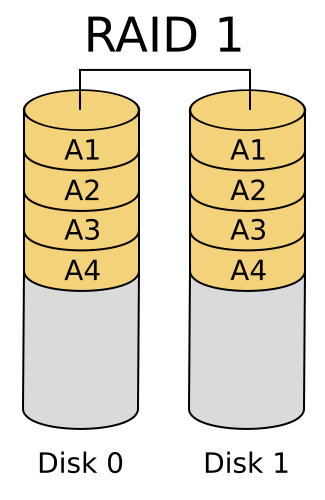
\includegraphics{RAID_1.svg}
\caption{RAID-1}
\end{figure}

\begin{itemize}
\item
  RAID-1 is commonly implemented with 2 disks, but RAID-1 sets can have
  any number of disks.
\item
  Read performance theoretically \texttt{n} times single disk.
\item
  Write performance is identical to a single disk in theory.
\end{itemize}

\subsubsection{RAID-1 fault tolerence}\label{raid-1-fault-tolerence}

RAID-1 maintains full data integrity with only a single disk remaining
functional:

\begin{itemize}

\item
  RAID-1 disk is identical to a single non-RAID disk.
\end{itemize}

In redundancy terms, RAID-1 is \texttt{N+(n-1)} redundant.

\subsubsection{RAID-1 storage
efficiency}\label{raid-1-storage-efficiency}

In RAID-1, data is mirrored onto all disks in the set. So only 1 disk's
worth of capacity in the set of \texttt{n} is useable, giving:

\begin{verbatim}
Efficiency(L=1, n) = 1 / n 
\end{verbatim}

\subsubsection{RAID-1 write penalty}\label{raid-1-write-penalty}

RAID-1 incurs a write for each disk in the set, so its write penalty is
\texttt{n}. Most RAID-1 sets have two disks, so this is often 2.

\section{Parity-based RAID}\label{parity-based-raid}

Parity relies on the XOR operation:

\begin{tabular}{@{}ccc@{}}
\toprule
A & B & C = A XOR B \$\tabularnewline
\midrule
0 & 0 & 0\tabularnewline
0 & 1 & 1\tabularnewline
1 & 0 & 1\tabularnewline
1 & 1 & 0\tabularnewline
\bottomrule
\end{tabular}

The parity blocks are computed bitwise from the data blocks using XOR.

\subsection{RAID-4}\label{raid-4}

RAID-4 stripes data blocks across \texttt{n-1} disks where the remaining
1 disk is used for parity. A minimum of 3 disks is required for RAID-4.

\begin{figure}
\centering
%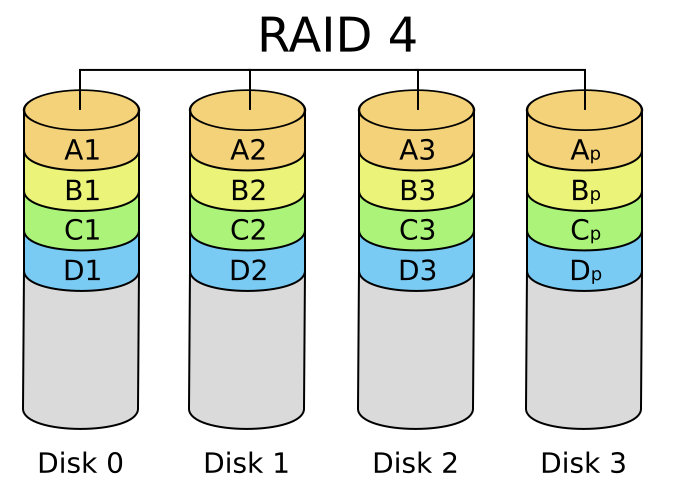
\includegraphics{RAID_4.svg}
\caption{RAID-4}
\end{figure}

Bit-by-bit the parity computation for a single stripe, in this case
\texttt{A} is:
\begin{align}
  A\_p & = A\_1 \oplus A\_2 \oplus A\_3 
\end{align}
The same parity computation is used for stripes $B, C, D$.

\subsection{RAID-5}\label{raid-5}

RAID-5 is conceptually similar to RAID-4. Parity is computed for each
stripe in the same way, but is stored differently. Instead of a single
parity disk, the parity blocks are distributed amongst all disks.

\begin{figure}
\centering
%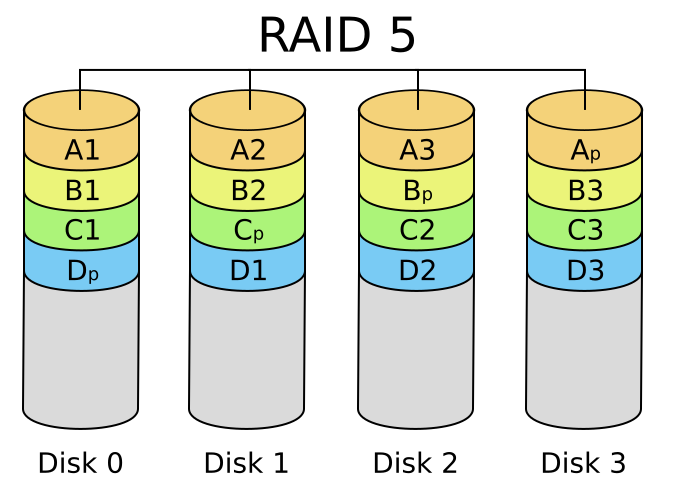
\includegraphics{RAID_5.svg}
\caption{RAID-5}
\end{figure}

\subsubsection{RAID-5 fault tolerence}\label{raid-5-fault-tolerence}

\begin{itemize}
\item
  RAID-5 is tolerent of failure of one disk. The array can continue to
  operate in degraded mode with no data loss and I/O operations
  available.
\item
  When the failed disk is replaced, a rebuild occurs onto the new disk
  by XORing the corresponding blocks on the remaining disks.
\item
  The array is vulnerable while degraded. If a second disk failure
  occurs, data will be lost.
\end{itemize}

In redundancy terms, RAID-5 is \texttt{N+1} redundant.

\subsubsection{RAID-5 storage
efficiency}\label{raid-5-storage-efficiency}

For RAID-5, the parity data takes up the capacity of one disk (although
distributed across them all). THe parity data does not contribute to the
storage available for use. This means that of the \texttt{n} disks in
the set, only the capacity equivalent to \texttt{n-1} disks is available
for use:

\begin{verbatim}
Efficiency(L=5, n)  =  ( n - 1 ) / n  =  1 - 1 / n 
\end{verbatim}

\subsection{RAID-6}\label{raid-6}

RAID-6 is similar to RAID-5 but adds a second parity block in each
stripe.

\begin{figure}
\centering
%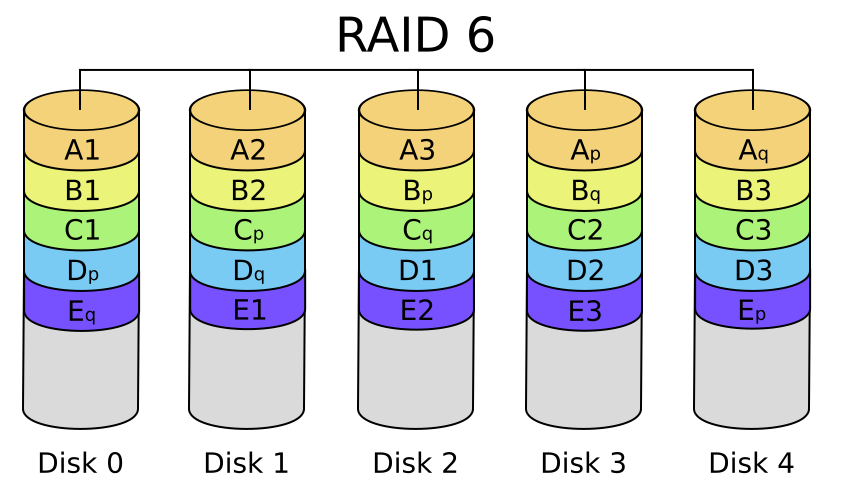
\includegraphics{RAID_6.svg}
\caption{RAID-6}
\end{figure}

\subsubsection{RAID-6 fault tolerence}\label{raid-6-fault-tolerence}

The second parity block in each stripe means that RAID-6 can sustain the
loss of up to two disks in a set while still remaining operational:

\begin{itemize}

\item
  Rebuild proceeds in the same way as RAID-5 except there are two parity
  blocks.
\end{itemize}

In redundancy terms, RAID-6 is \texttt{N+2} redundant.

\subsubsection{RAID-6 storage
efficiency}\label{raid-6-storage-efficiency}

In RAID-6 we lose the equivalent of two disks' space to store the parity
information.

\begin{verbatim}
Efficiency(L=6, n)  =  ( n - 2 ) / n  =  1 - 2 / n 
\end{verbatim}

\section{Nested RAID}\label{nested-raid}

\subsection{RAID-01}\label{raid-01}

\begin{figure}
\centering
%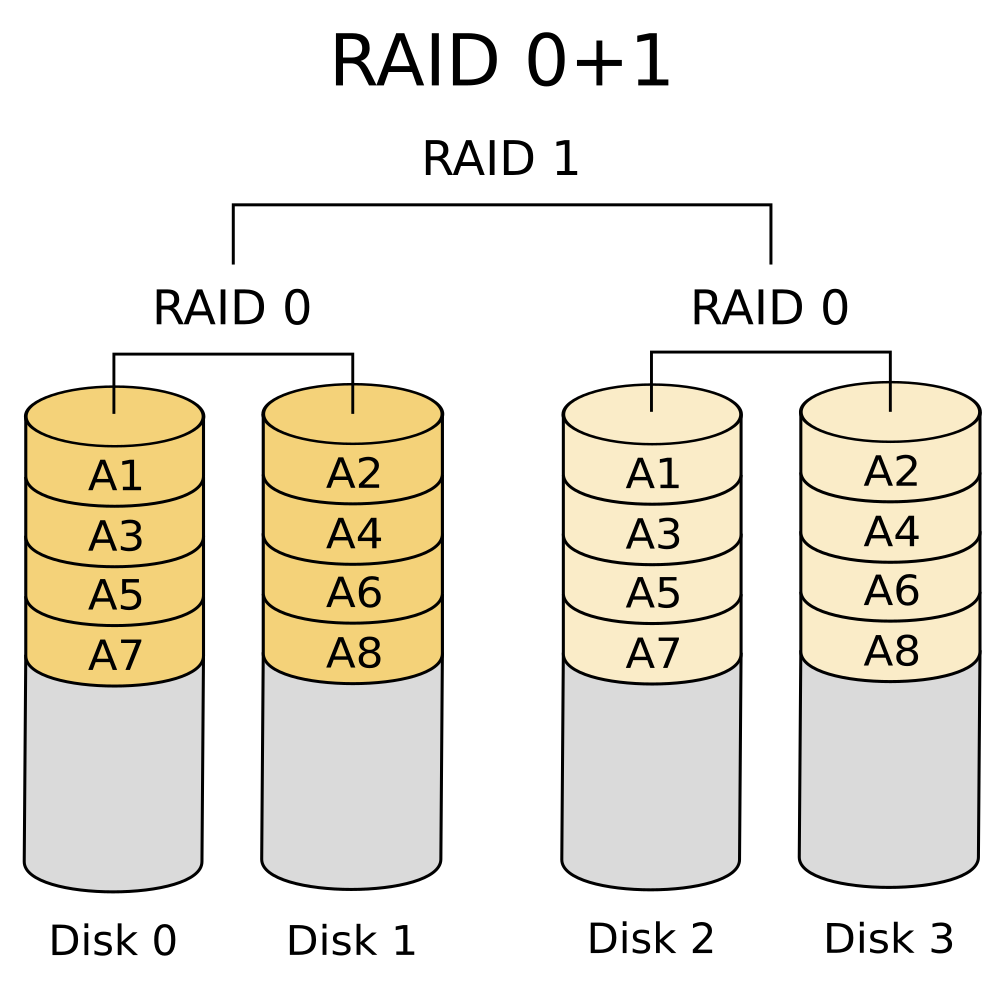
\includegraphics{RAID_nested_01.svg}
\caption{RAID-01}
\end{figure}

\subsection{RAID-10}\label{raid-10}

\begin{figure}
\centering
%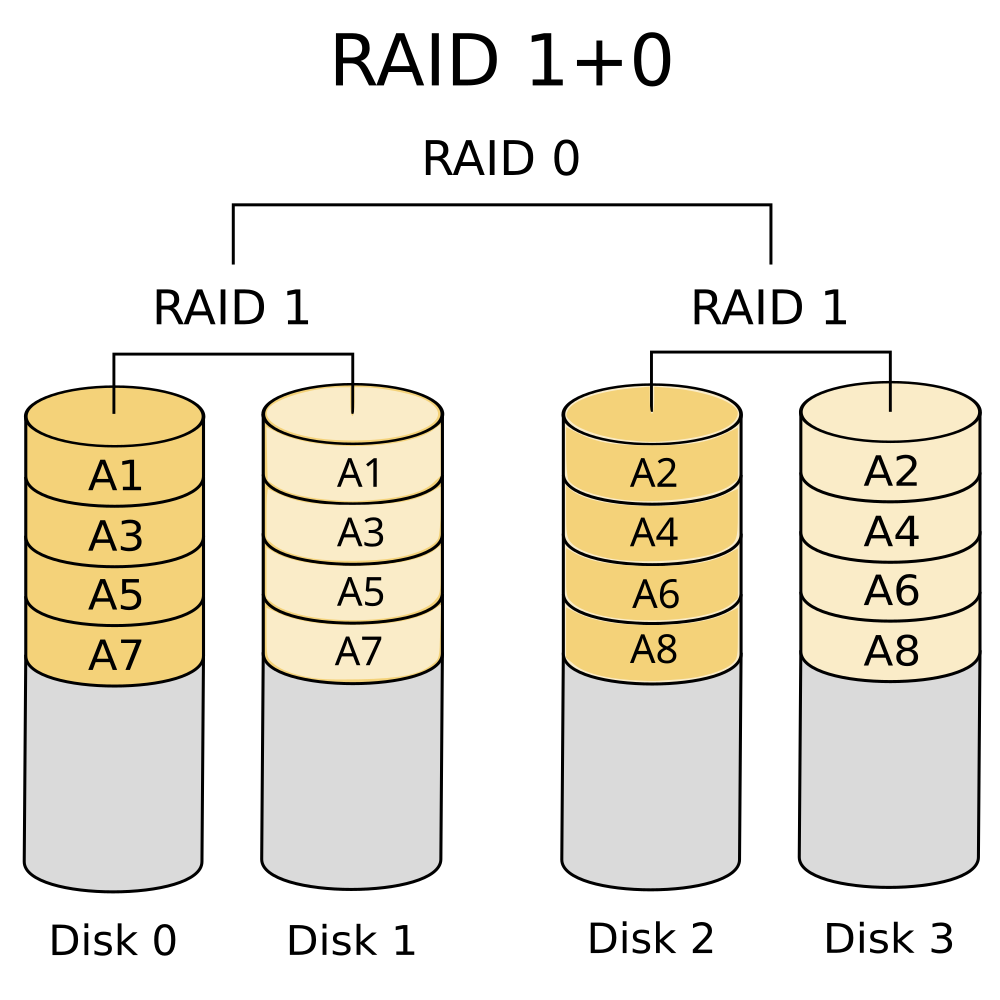
\includegraphics{RAID_nested_10.svg}
\caption{RAID-10}
\end{figure}

\section{Implementation}\label{implementation}

RAID can be implemented in either software or hardware:

\begin{description}
\item[Hardware-based]
RAID is where the Host Bus Adapter (HBA) implements the RAID
functionality. The host and its OS sees the single block device
resulting from the RAID implementation.
\item[Software-based]
RAID is where the RAID functionality is implemented within the host,
usually as part of the operating system. The HBA just passes through
each physical disk as a block device.
\item[Hybrid]
RAID is sometimes used for nested RAID configurations. Disks are
combined into RAID sets by one or more HBAs and the exported block
devices are then grouped into RAID set(s) in software.
\item[Hardware-assisted]
RAID is a mix of hardware and software RAID. The XOR computations are
accelerated by a chip in the HBA while the rest of the RAID
implementation is done in software. Seen in some motherboard-based RAID
controllers and often best avoided!
\end{description}

Despite a lot of ill-informed comment online and elsewhere, it is almost
impossible to definitively say whether software or hardware-based RAID
is preferable. The choice depends on a large number of factors: devices,
HBA capabilities, HBA throughput, OS, filesystem(s) to be used,
portability requirements.

\section{Monitoring}\label{monitoring}

\textbf{Problem:} RAID set becomes degraded due to disk failure.
Essential that the failed disk is replaced before a further failure
occurs.

\textbf{Solution:} The RAID set must have appropriate monitoring
installed.

\begin{itemize}
\item
  Hardware RAID controllers often have a separate management
  capabilities, appearing as a separate device on the host system. This
  often needs proprietary software to work.
\item
  Software RAID setups more visible by default to the OS and will appear
  in system logs.
\item
  Either way, should be proactively sending notifications (e.g.~e-mail,
  helpdesk API).
\end{itemize}

\section{Hot spares}\label{hot-spares}

If hardware / software capabilities and available drive bays allow, it
is possible to automatically replace a failed disk with a hot spare.

\begin{enumerate}
\def\labelenumi{\arabic{enumi}.}
\item
  The RAID controller / software detects the failed disk, sends
  notification.
\item
  Controller removes it from the array (which is now degraded). The disk
  remains physically in its bay and plugged into the same port.
\item
  The controller/software then adds the hot spare to the array. Re-build
  commences on to the hot spare.
\item
  Array is then in a healthy state once rebuild has completed.
\item
  Failed disk can be replaced on schedule on next physical visit.
  Re-built onto replaced disk, hot spare removed from array.
\end{enumerate}
